\begin{frame}{Game setup and data extraction}
\begin{itemize}
\item Basic 5x5 game setup
\begin{itemize}
\item A game consists of 10 summoners, 5 on each team, each summoner selects a champion to play on a lane, the summon also selects which summoners spells, runes and masteries the summoner want to help boost the champion selected.   
\item Lanes: \{top, middel, jungle, bottom\}
\item Summoner(player): \{level ,champion, summoner spells, runes, masteries\}
\item Champion: \{level, passive, 3 tallents, 1 ulti, items\}
\end{itemize}
\end{itemize}
\vspace{20cm}
\end{frame}
\begin{frame}{Champion example}
\begin{figure}[h!]
\centering
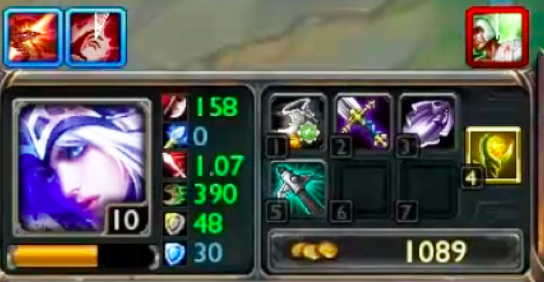
\includegraphics[width=4cm]{leagueoflegends/ashe1}
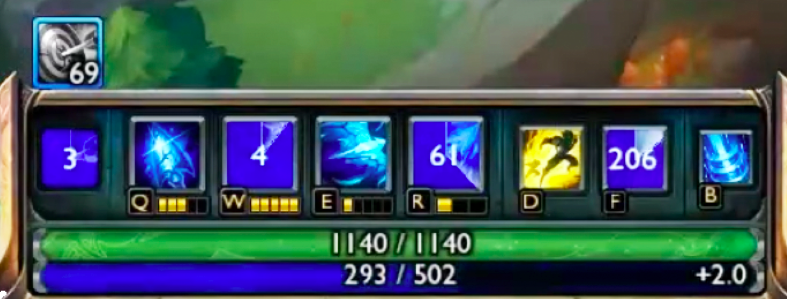
\includegraphics[width=4cm]{leagueoflegends/ashe2}
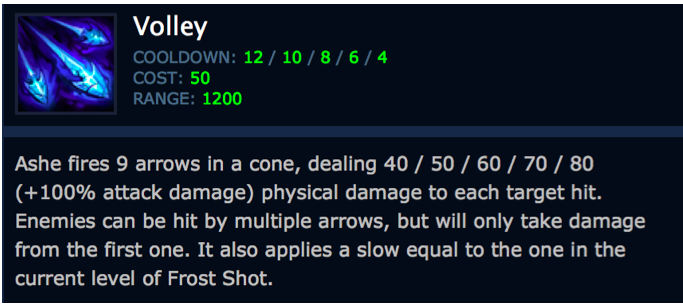
\includegraphics[width=4cm]{leagueoflegends/volly}
\caption{Ashe's stats and spells}
\end{figure}
\end{frame}
\begin{frame}{Match objectives}
\begin{itemize}
\item Nesus, one for each team 
\item Inhibitor 3 for each team 
\item Tower 11 for each team 
\item Baron 1 in total
\item Dragon 1 in total
\item Gold and experience
\item Killing enermies, minions and monsters 
\end{itemize}
\end{frame}
\begin{frame}{Map}
\begin{figure}[h!]
\centering
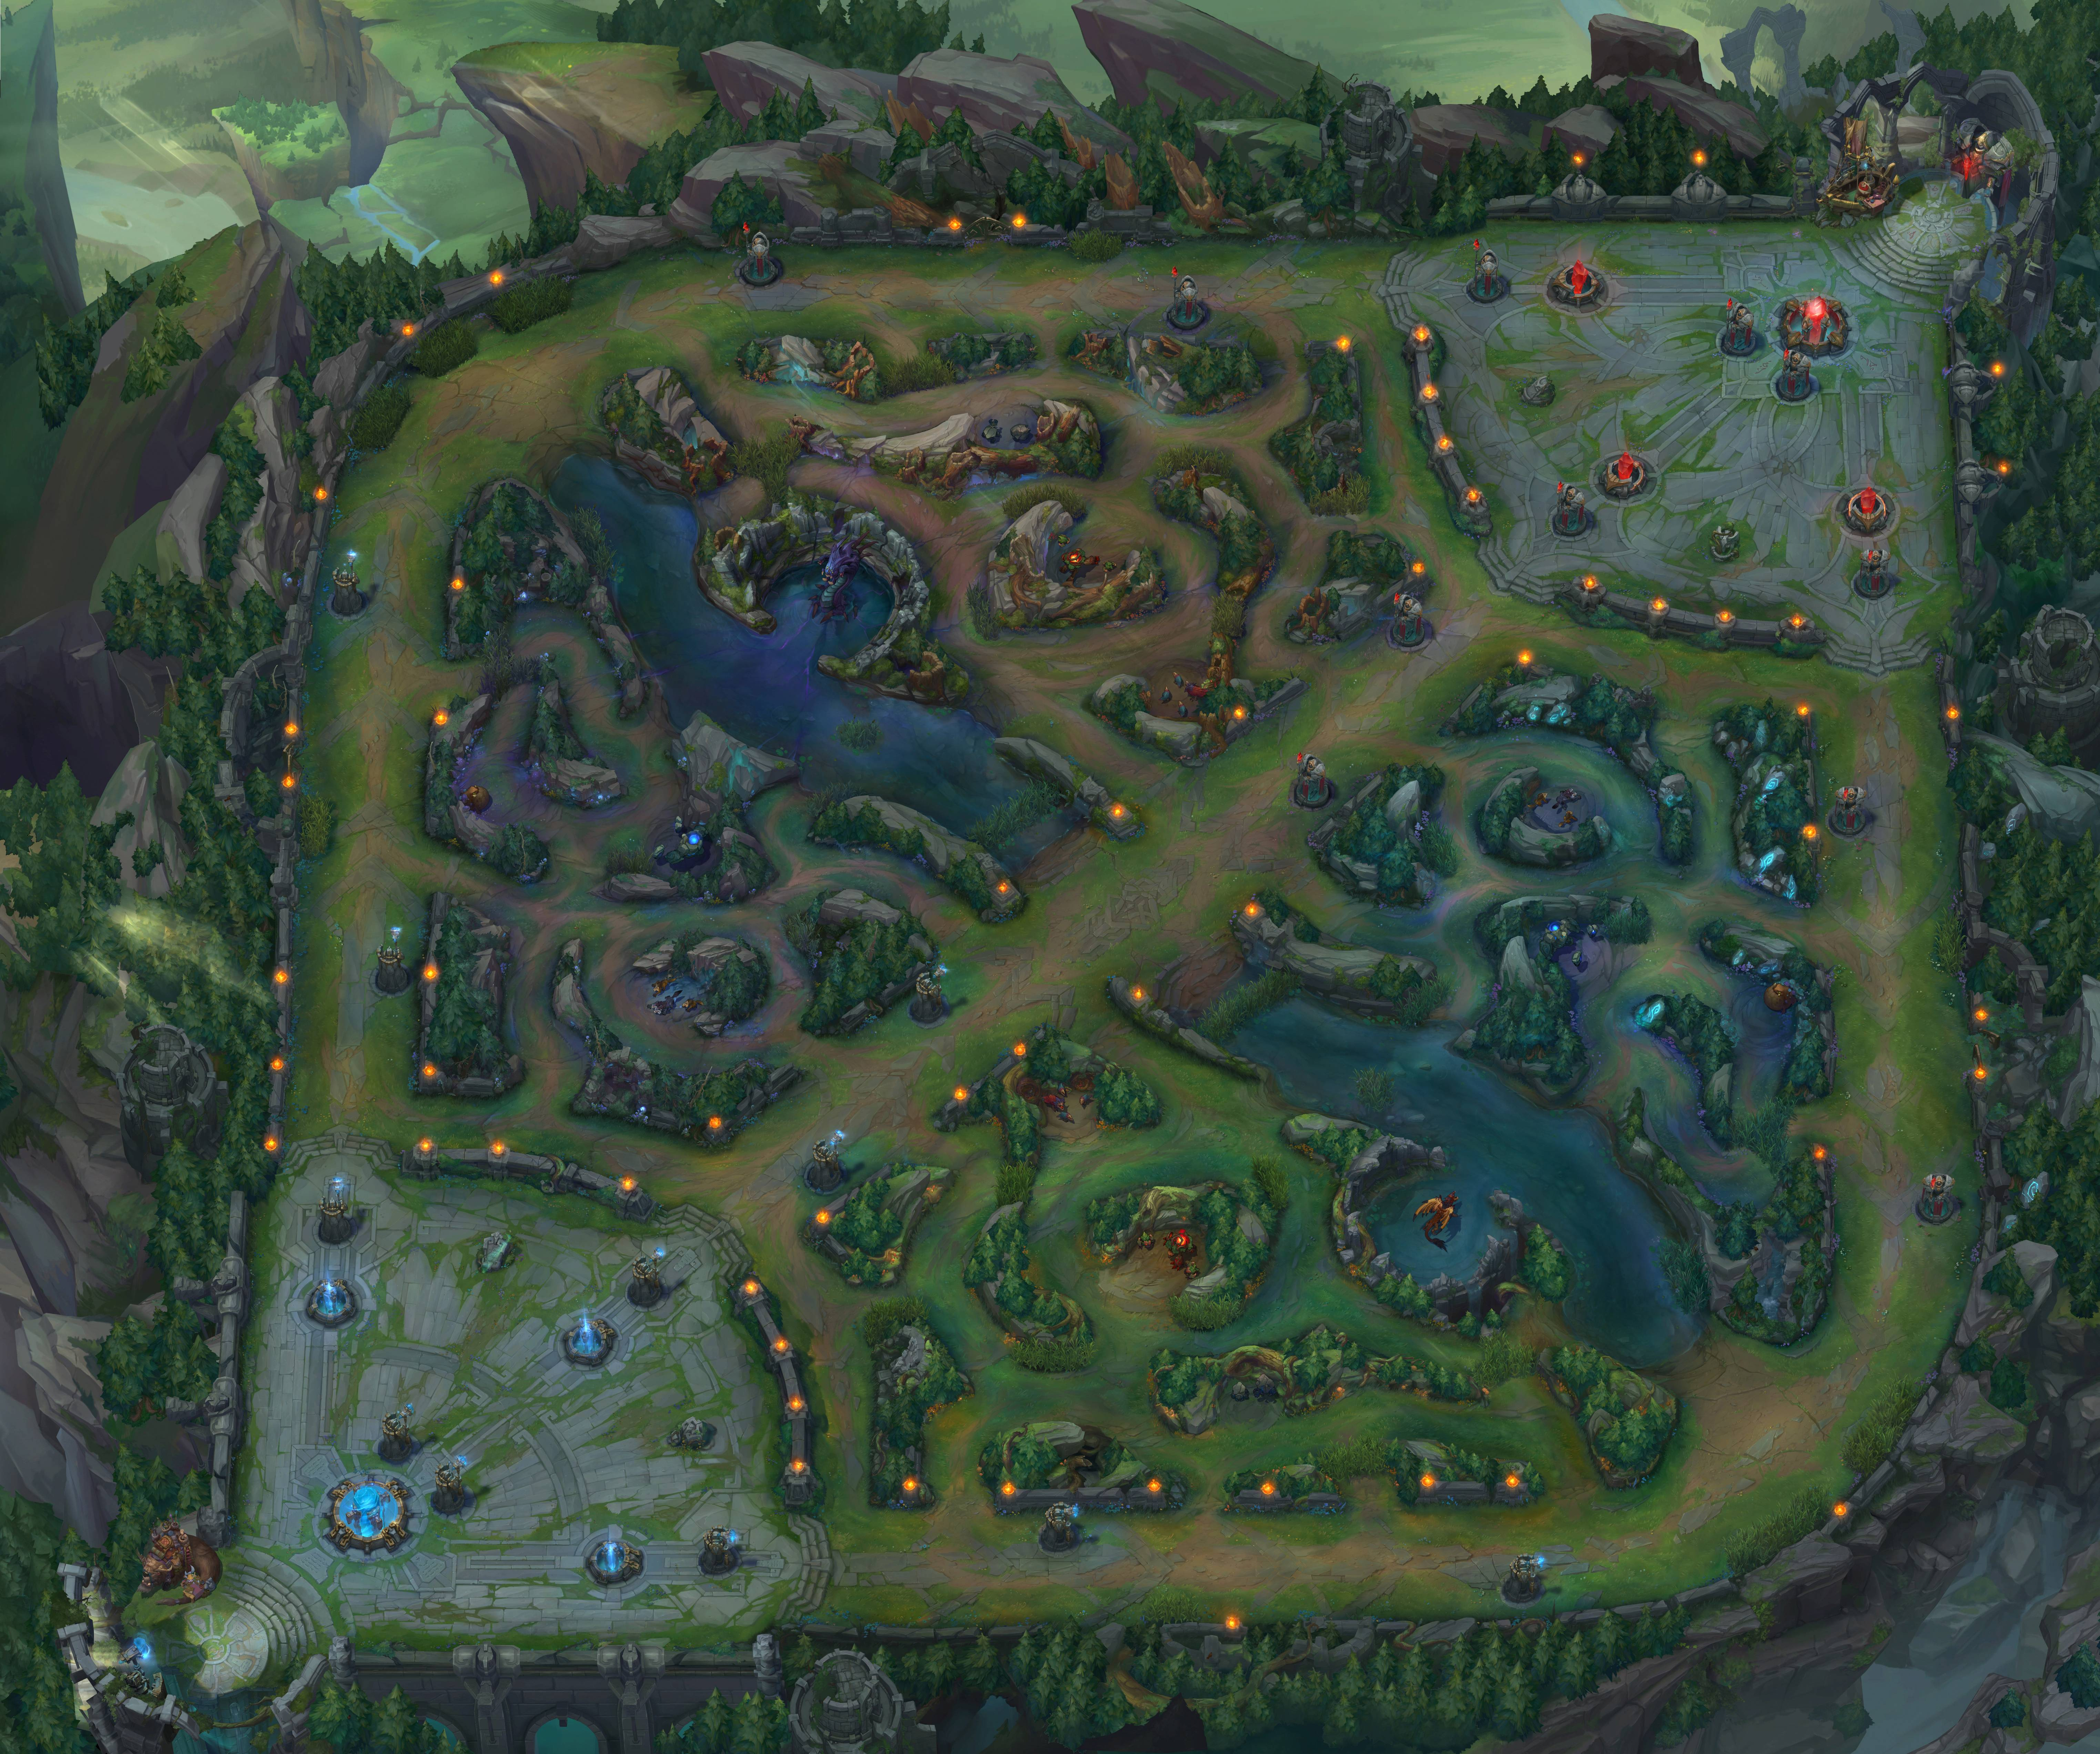
\includegraphics[width=\linewidth, height=\textheight]{leagueoflegends/map}
\caption{Map of a classical 5x5 match}
\end{figure}
\end{frame}
\begin{frame}{API and data}
\begin{itemize}
\item Riot games API
\begin{itemize}
\item All match data is available through riot games api. 
\item Website: https://developer.riotgames.com/
\item Path: /api/lol/\{region\}/v2.2/match/\{matchId\}
\item match-v2.2 is used for data extraction 
\end{itemize}
\item Data 
\begin{itemize}
\item Json 
\item Path parameters: \{region, matchid\}
\item Query parameter: \{includeTimeline\} 
\end{itemize}
\end{itemize}
\end{frame}
\begin{frame}{Data object example}
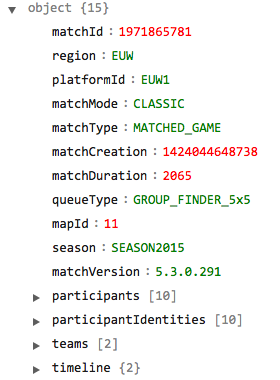
\includegraphics[scale=0.5]{leagueoflegends/gameobject}
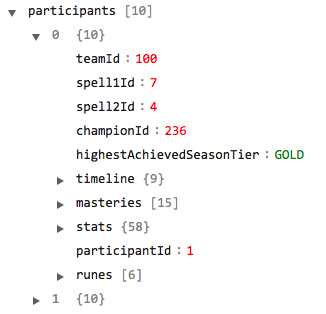
\includegraphics[scale=0.5]{leagueoflegends/participant}
\end{frame}
\begin{frame}[fragile]{Data filtering}
\newminted{python}{fontsize=\footnotesize}
\begin{minted}{python}
 MatchFilter({"matchMode": ["CLASSIC"],
    "matchType": ["MATCHED_GAME"],
    "queueType": ["NORMAL_5x5_BLIND", "RANKED_SOLO_5x5", "RANKED_PREMADE_5x5",
       "NORMAL_5x5_DRAFT", "RANKED_TEAM_5x5",  "GROUP_FINDER_5x5"],
    "participants->*->timeline->xpPerMinDeltas->*": ["!0"]})
\end{minted}
\end{frame}